\documentclass{article}

\usepackage[utf8]{inputenc}
\usepackage{enumitem}
\usepackage{latexsym}
\usepackage{amsfonts}
\usepackage{amsmath,amssymb,amsthm}
\usepackage{amsfonts}
\usepackage{parskip}
\usepackage{listings}

\usepackage{tikz}
\usetikzlibrary{arrows, automata, bending, positioning}

\title{Homework 1}
\author{Asier Garcia Ruiz}

\begin{document}
\maketitle

\newenvironment{question}[2]
{
    {\large \textbf{Question #1.}}\\
    #2\\\\
}{\newpage}
\begin{question}{1}{
        Give the state diagrams for the DFA's that accept the following languages:
    }
    a) (4 points) $L = \{x | x
        \text{ is a binary string, which, when interpreted as a binary number, is equivalent to } 3 \mod 6\}$
    \\
    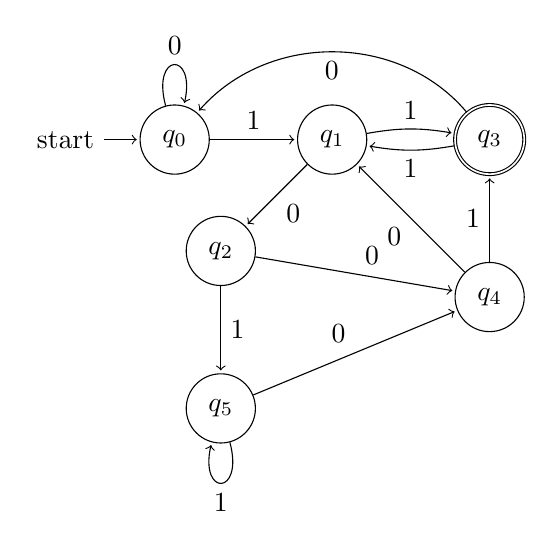
\begin{tikzpicture}[shorten >=1pt,node distance=2cm,on grid,auto]

        \node[state, initial]   (q_0)                       {$q_0$};
        \node[state]            (q_1) [right=of q_0]        {$q_1$};
        \node[state]            (q_2) [below left=of q_1]   {$q_2$};
        \node[state, accepting] (q_3) [right=of q_1]        {$q_3$};
        \node[state]            (q_4) [below=of q_3]        {$q_4$};
        \node[state]            (q_5) [below=of q_2]        {$q_5$};

        \path[->]   (q_0) edge [loop above] node {0} ()
        edge node {1} (q_1)
        (q_1) edge node {0} (q_2)
        edge [bend left=10] node {1} (q_3)
        (q_2) edge node {0} (q_4)
        edge node {1} (q_5)
        (q_3) edge [bend right=50] node {0} (q_0)
        edge [bend left=10] node {1} (q_1)
        (q_4) edge node {0} (q_1)
        edge node {1} (q_3)
        (q_5) edge node {0} (q_4)
        edge [loop below] node {1} ()
        ;
    \end{tikzpicture}

    b) (4 points) $L = \{x | x
        \text{ is a binary string which contains an even number of 1’s and ends in 010}\}$
    \\
    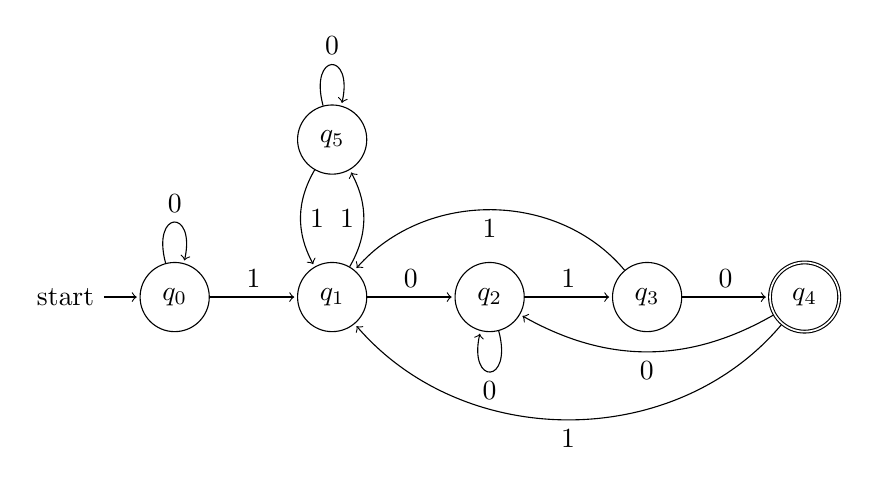
\begin{tikzpicture}[shorten >=1pt,node distance=2cm,on grid,auto]
        \node[state, initial]   (q_0)                   {$q_0$};
        \node[state]            (q_1) [right=of q_0]    {$q_1$};
        \node[state]            (q_2) [right=of q_1]    {$q_2$};
        \node[state]            (q_3) [right=of q_2]    {$q_3$};
        \node[state, accepting] (q_4) [right=of q_3]    {$q_4$};
        \node[state]            (q_5) [above=of q_1]    {$q_5$};

        \path[->] (q_0) edge [loop above] node {0} ()
        edge node {1} (q_1)
        (q_1) edge node {0} (q_2)
        (q_1) edge [bend right=30] node {1} (q_5)
        (q_2) edge [loop below] node {0} ()
        (q_2) edge node {1} (q_3)
        (q_3) edge node {0} (q_4)
        (q_3) edge [bend right=50] node {1} (q_1)
        (q_4) edge [bend left=30] node {0} (q_2)
        (q_4) edge [bend left=50] node {1} (q_1)
        (q_5) edge [loop above] node {0} ()
        (q_5) edge [bend right=30] node {1} (q_1)
        ;
    \end{tikzpicture}
\end{question}

\begin{question}{2}{
        Let $ONE-OR-ALL(L_1, L_2, L_3)$ be the set which contains all strings which are
        either members of all three languages $L_1, L_2, L_3$ or are contained in
        \emph{exactly} one of the three languages. Show that, if $L_1, L_2$, and $L_3$ are
        regular, then $ONE-OR-ALL(L_1, L_2, L_3)$ is also regular.
    }
    We assume that $L_1, L_2$ and $L_3$ are all regular. This implies they are all
    closed under complement, intersection, union, difference, and symmetric
    difference. We have that
    \[ONE-OR-ALL(L_1, L_2, L_3) = L_1 \oplus L_2 \oplus L_3.\]
    Thus, $ONE-OR-ALL(L_1, L_2, L_3)$ is regular.
\end{question}

\begin{question}{3}{
        Let $L[0]$ be defined formally as $\{x_10x_2...0x_n | x_i \in \Sigma, x_1...x_n\in L\}$.
        In other words, strings of $L[0]$ are formed by taking a string from $L$
        and inserting a $0$ between each character of the word, so that if $L = \{11,1010\}$,
        then $L[0] = \{101, 1000100\}$.  Prove that if $L$ is regular, so is $L[0]$.
    }
    Let $M := (Q_1, \Sigma, \delta, q_0, F)$ be an automaton that recognises $L$. We will
    make an automaton $M' := (Q', \Sigma', \delta', q_0', F')$ that recognises $L[0]$. Now let
    $Q_2 := \{q_i | i \in 1,...,n-1\}, n = |Q_1|$, and $Q' = Q_1 \cup Q_2$. So we have added $n-1$
    intermediate states. We let $\Sigma' := \Sigma$, $q_0' := q_0$, and $F' := F$.
    Now, let $a \in Q'$, $r_i \in Q_1$ and $s_i \in Q_2$. We define $\delta'$ as follows:
    \begin{align*}
        \delta'(r_i, 0) & = s_i,            \\
        \delta'(s_i, a) & = \delta(r_i, a).
    \end{align*}
    Basically, there is a state in $Q_2$ to which we can transition to on a 0.
    This state is in between each
    of the original states. Once we get to that state, the transition function will use the
    "original" decision (i.e. $\delta(r_i, a)$) to move on to the next state.

    We have now created a new automaton $M'$ that will accept $L[0]$, thus $L[0]$ is a
    regular language.
\end{question}


\end{document}